\documentclass[pdflatex,compress,mathserif]{beamer}

%\usetheme[dark,framenumber,totalframenumber]{ElektroITK}
\usetheme[darktitle,framenumber,totalframenumber]{ElektroITK}

\usepackage[utf8]{inputenc}
\usepackage[T1]{fontenc}
\usepackage{lmodern}
\usepackage[bahasai]{babel}
\usepackage{amsmath}
\usepackage{amsfonts}
\usepackage{amssymb}
\usepackage{graphicx}
\usepackage{multicol}
\usepackage{lipsum}
\usefonttheme[onlymath]{serif}

\newcommand*{\Scale}[2][4]{\scalebox{#1}{$#2$}}%

\setbeamertemplate{caption}[numbered]

\title{MATEMATIKA DASAR}
\subtitle{Persamaan Linear dan Kuadratik}

\author{Mifta Nur Farid}

\begin{document}

\maketitle

\section{Persamaan}

\begin{frame}
\frametitle{Persamaan}
	\begin{itemize}
		\item Secara umum suatu persamaan adalah pernyataan dari dua buah ekspresi matematika yang bernilai sama.
		$$ 4 + 3 = 2 + 5 $$
		\item Dalam permasalahan yang akan dipelajari lebih lanjut akan mengandung suatu variabel, yang bisa dinyatakan dalam suatu simbol (biasanya dalam huruf) yang menyatakan suatu bilangan.
		$$ 4x+6 = 18 $$
		\item Nilai $x$ yang memenuhi persamaan tersebut disebut solusi atau akar dari persamaan.
	\end{itemize}
\end{frame}

\begin{frame}
	\frametitle{Persamaan}
	\begin{center}
		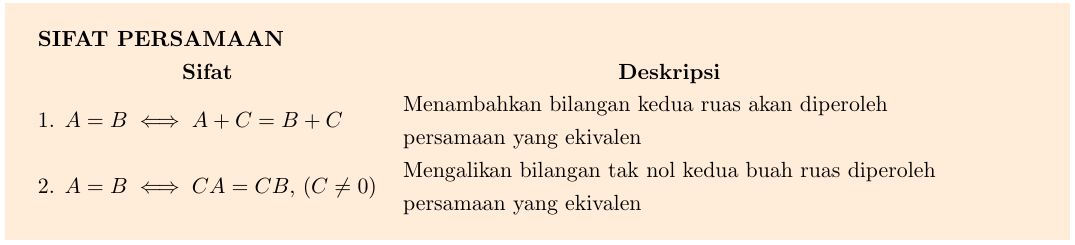
\includegraphics[width=\linewidth]{img/img01}
	\end{center}
\end{frame}

\section{Solusi Persamaan Linear}

\begin{frame}
	\frametitle{Solusi Persamaan Linear}
	\begin{center}
		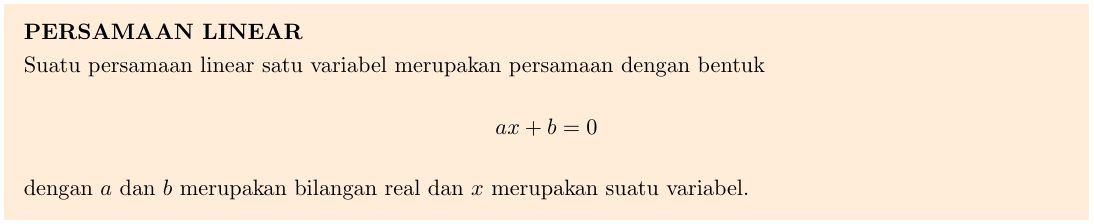
\includegraphics[width=\linewidth]{img/img02}
		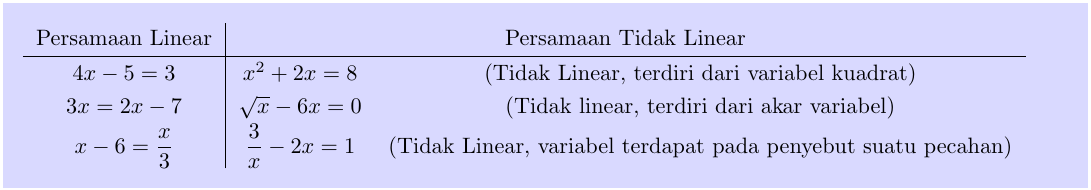
\includegraphics[width=\linewidth]{img/img03}
	\end{center}
\end{frame}

\begin{frame}
	\frametitle{Solusi Persamaan Linear}
	\begin{center}
		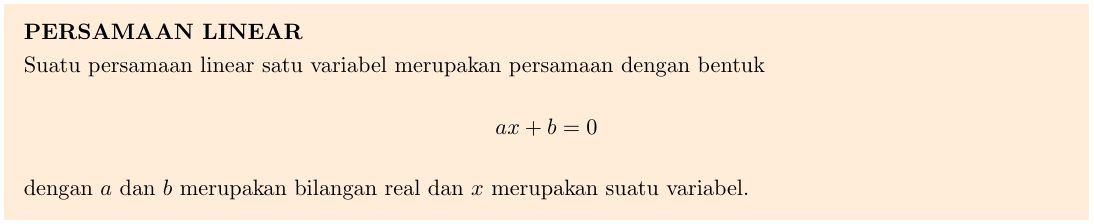
\includegraphics[width=\linewidth]{img/img02}
		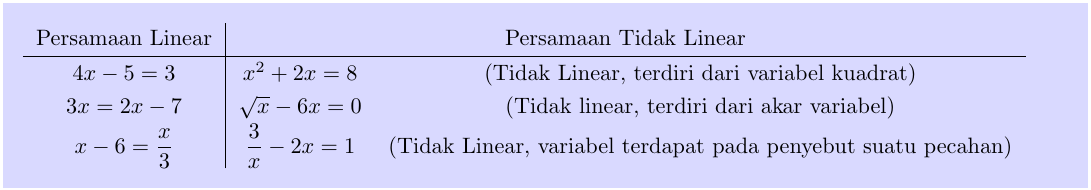
\includegraphics[width=\linewidth]{img/img03}
	\end{center}
\end{frame}

\begin{frame}
	\frametitle{Solusi Persamaan Linear}
	\begin{center}
		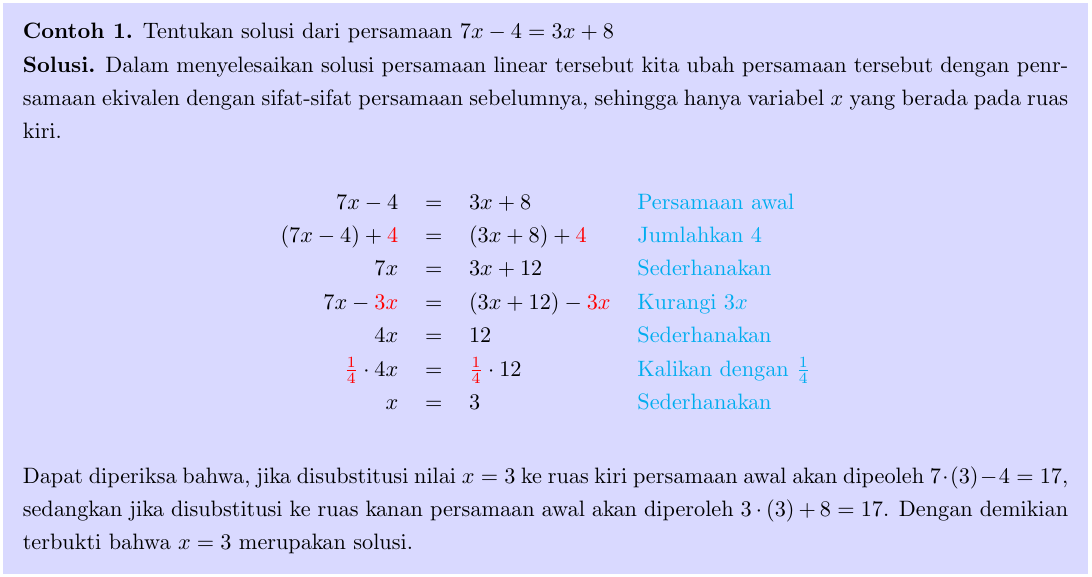
\includegraphics[width=\linewidth]{img/img04}
	\end{center}
\end{frame}


\begin{frame}
	\frametitle{Solusi Persamaan Linear}
	\begin{center}
		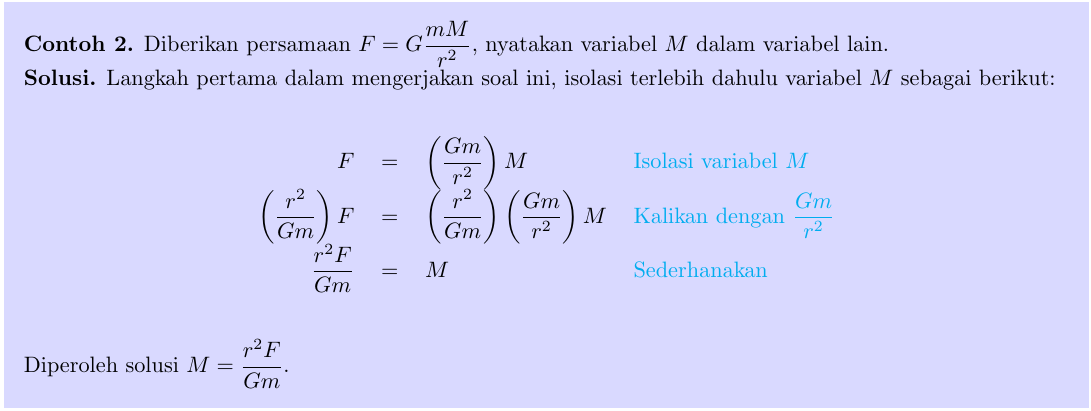
\includegraphics[width=\linewidth]{img/img05}
	\end{center}
\end{frame}

\begin{frame}
	\frametitle{Solusi Persamaan Linear}
	\begin{center}
		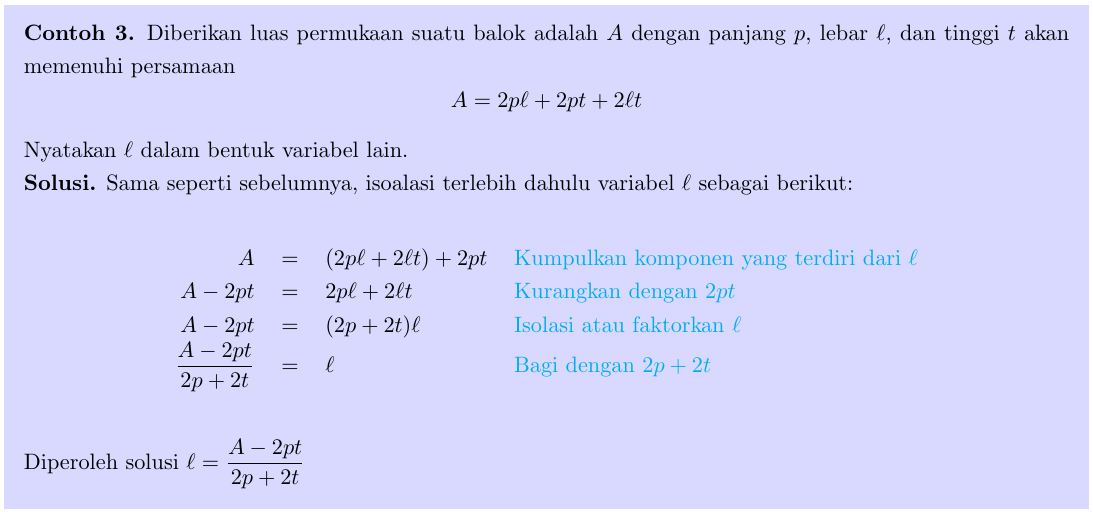
\includegraphics[width=\linewidth]{img/img06}
	\end{center}
\end{frame}

\section{Solusi Persamaan Kuadratik}

\begin{frame}
	\frametitle{Solusi Persamaan Kuadratik}
	\begin{center}
		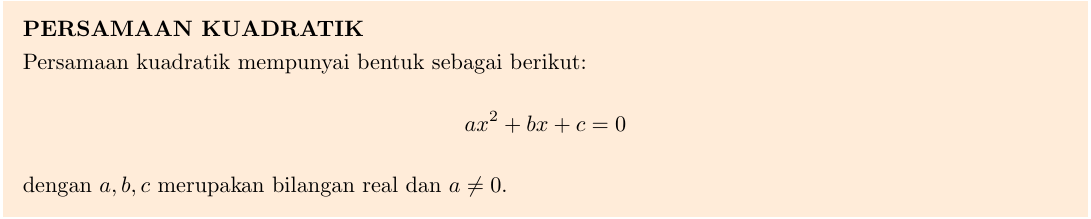
\includegraphics[width=\linewidth]{img/img07}
	\end{center}
\end{frame}

\subsection{Metode Faktor}

\begin{frame}
	\frametitle{Metode Faktor}
	\begin{center}
		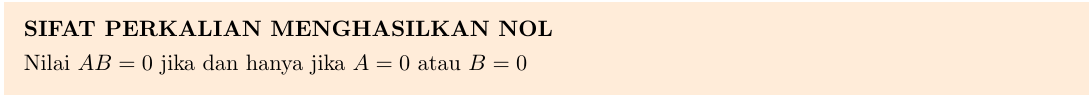
\includegraphics[width=\linewidth]{img/img08}
	\end{center}
\end{frame}

\begin{frame}
	\frametitle{Metode Faktor}
	\begin{center}
		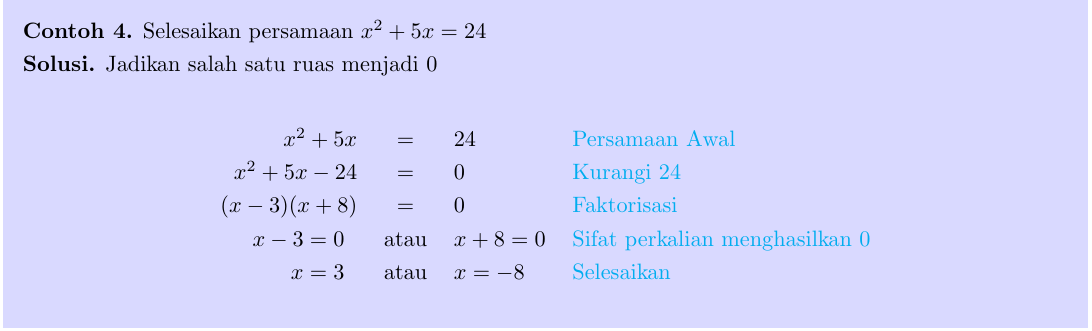
\includegraphics[width=\linewidth]{img/img09}
	\end{center}
\end{frame}

\begin{frame}
	\frametitle{Metode Faktor}
	\begin{center}
		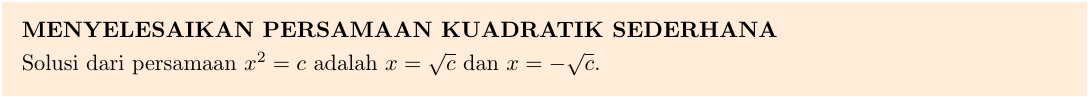
\includegraphics[width=\linewidth]{img/img10}
	\end{center}
\end{frame}

\begin{frame}
	\frametitle{Metode Faktor}
	\begin{center}
		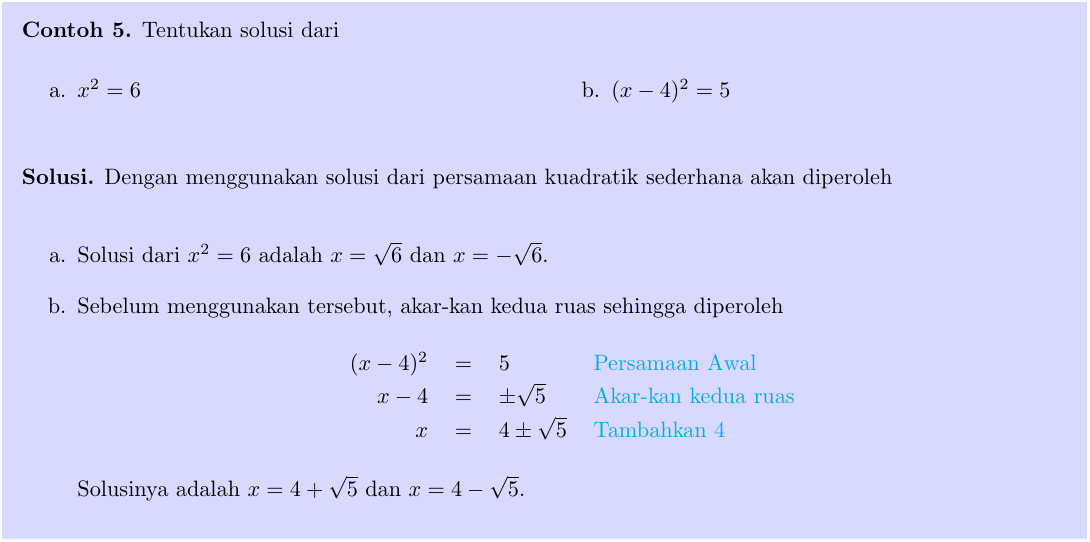
\includegraphics[width=\linewidth]{img/img11}
	\end{center}
\end{frame}

\subsection{Melengkapi Kuadrat Sempurna}

\begin{frame}
	\frametitle{Melengkapi Kuadrat Sempurna}
	\begin{center}
		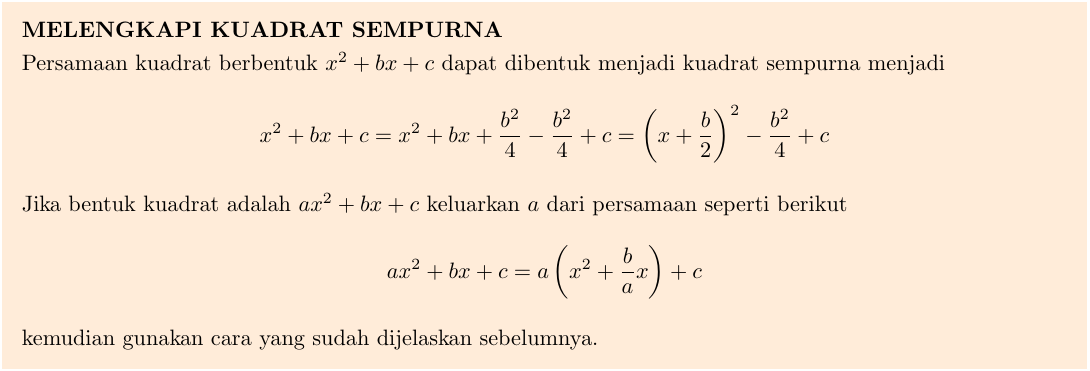
\includegraphics[width=\linewidth]{img/img12}
	\end{center}
\end{frame}

\begin{frame}
	\frametitle{Melengkapi Kuadrat Sempurna}
	\begin{center}
		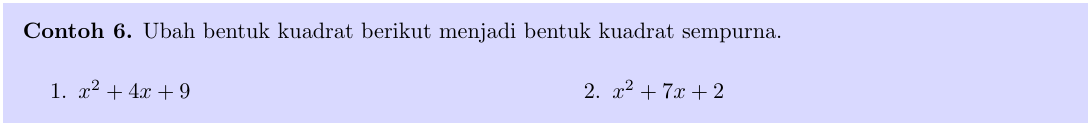
\includegraphics[width=\linewidth]{img/img13}
		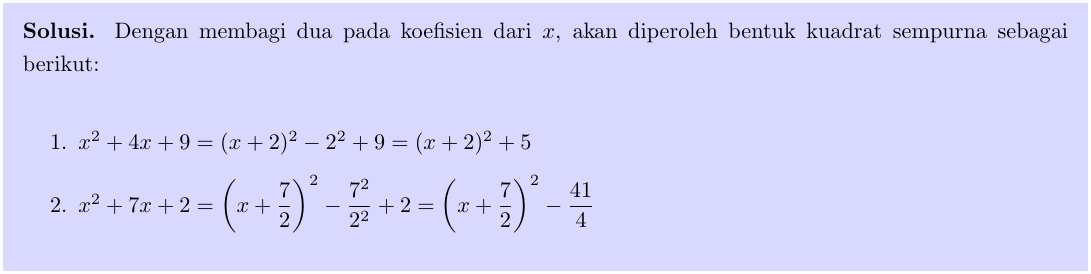
\includegraphics[width=\linewidth]{img/img14}
	\end{center}
\end{frame}

\begin{frame}
	\frametitle{Melengkapi Kuadrat Sempurna}
	\begin{center}
		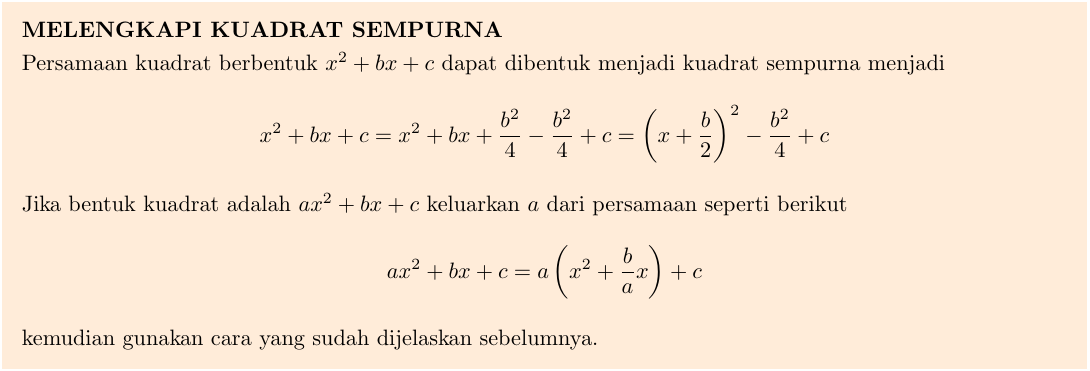
\includegraphics[width=\linewidth]{img/img12}
	\end{center}
\end{frame}


\begin{frame}
	\frametitle{Melengkapi Kuadrat Sempurna}
	\begin{center}
		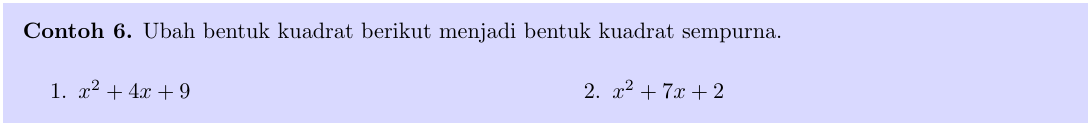
\includegraphics[width=\linewidth]{img/img13}
	\end{center}
\end{frame}


\begin{frame}
	\frametitle{Melengkapi Kuadrat Sempurna}
	\begin{center}
		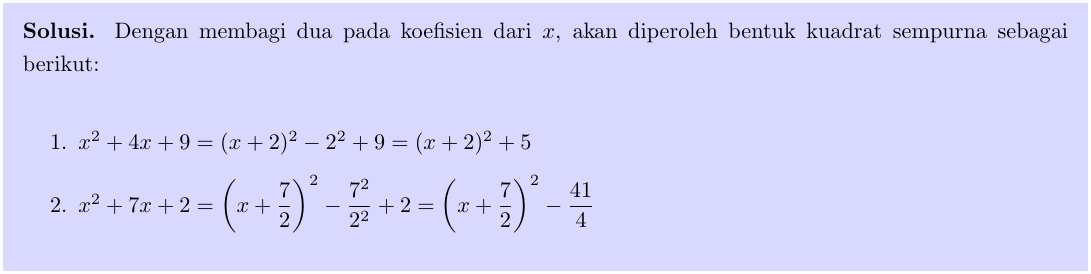
\includegraphics[width=\linewidth]{img/img14}
	\end{center}
\end{frame}


\begin{frame}
	\frametitle{Melengkapi Kuadrat Sempurna}
	\begin{center}
		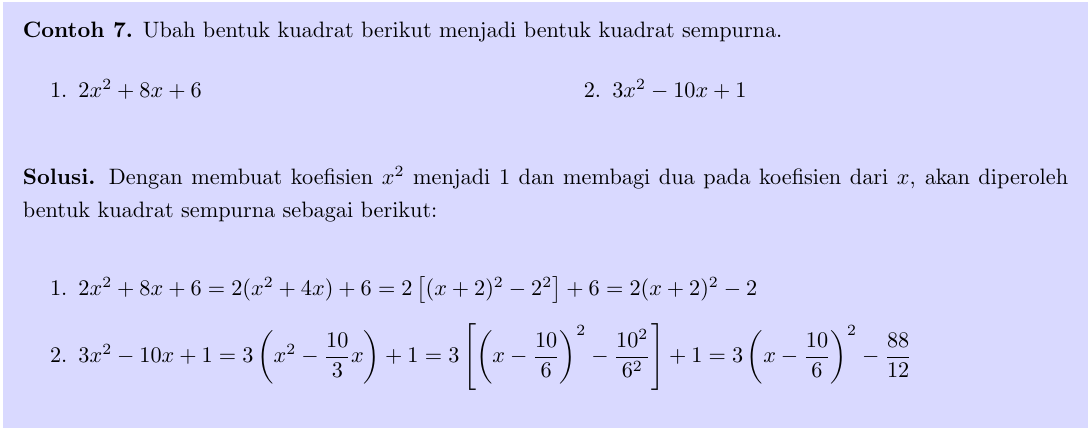
\includegraphics[width=\linewidth]{img/img15}
	\end{center}
\end{frame}


\begin{frame}
	\frametitle{Melengkapi Kuadrat Sempurna}
	\begin{center}
		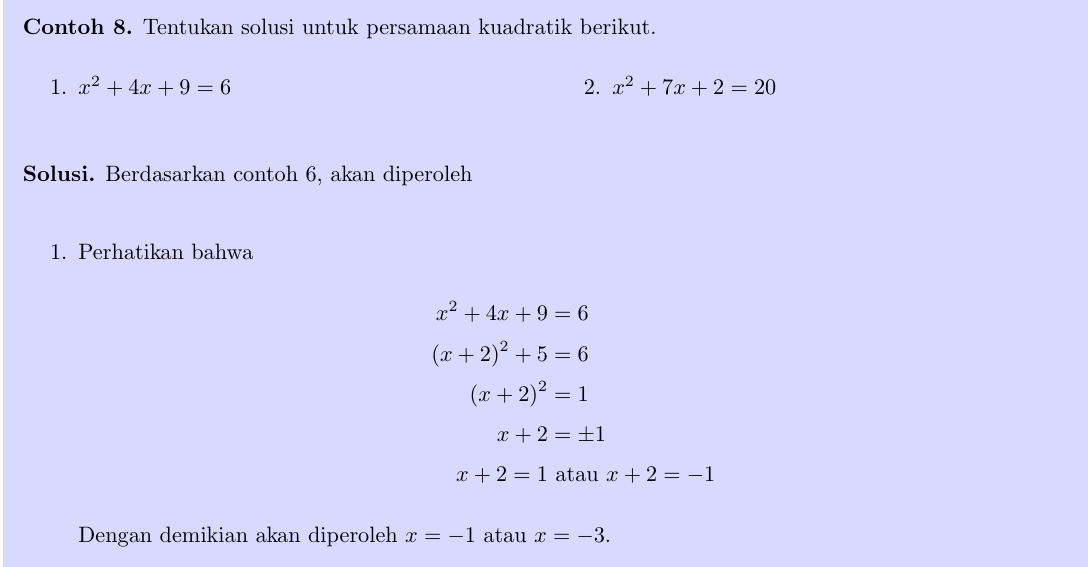
\includegraphics[width=\linewidth]{img/img16}
	\end{center}
\end{frame}


\begin{frame}
	\frametitle{Melengkapi Kuadrat Sempurna}
	\begin{center}
		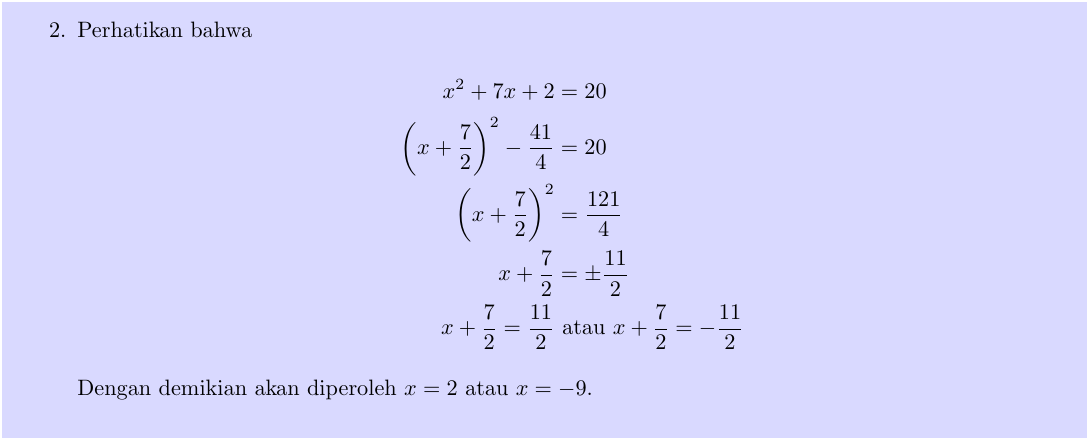
\includegraphics[width=\linewidth]{img/img17}
	\end{center}
\end{frame}


\begin{frame}
	\frametitle{Melengkapi Kuadrat Sempurna}
	\begin{center}
		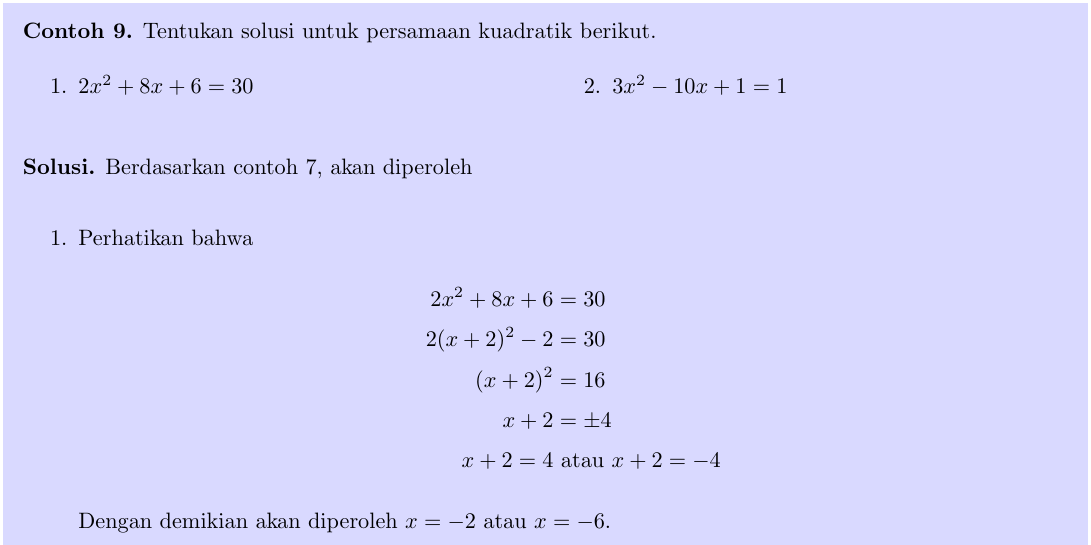
\includegraphics[width=\linewidth]{img/img18}
	\end{center}
\end{frame}

\begin{frame}
	\frametitle{Melengkapi Kuadrat Sempurna}
	\begin{center}
		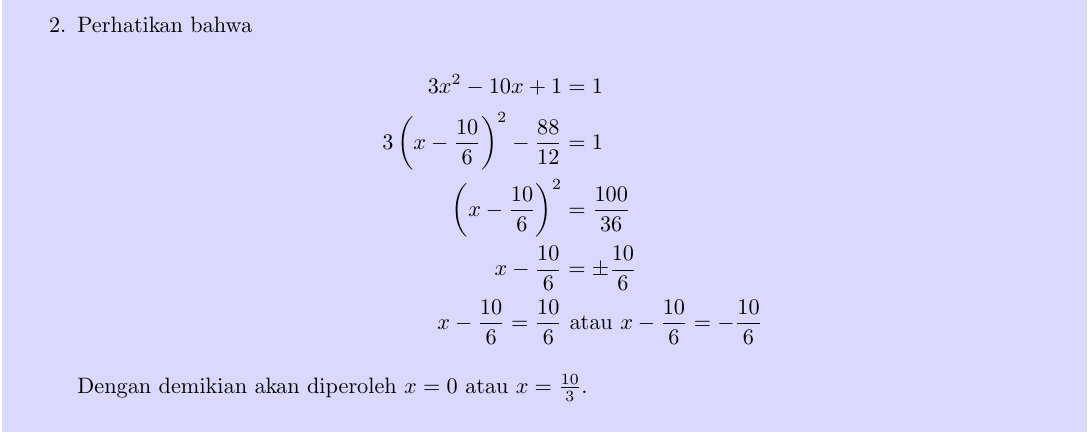
\includegraphics[width=\linewidth]{img/img19}
	\end{center}
\end{frame}

\subsection{Rumus Persamaan Kuadrat}

\begin{frame}
	\frametitle{Rumus Persamaan Kuadrat}
	\begin{center}
		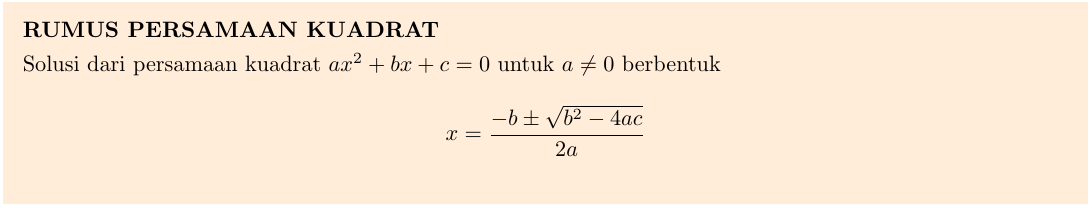
\includegraphics[width=\linewidth]{img/img20}
	\end{center}
\end{frame}

\begin{frame}
	\frametitle{Rumus Persamaan Kuadrat}
	\begin{center}
		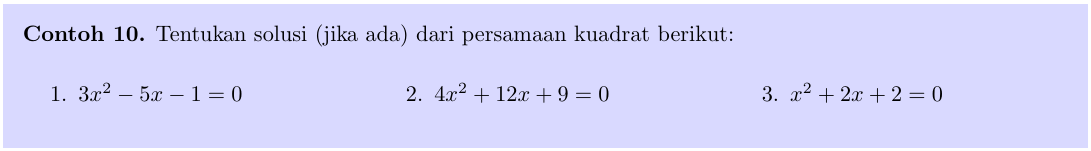
\includegraphics[width=\linewidth]{img/img21}
	\end{center}
\end{frame}

\begin{frame}
	\frametitle{Rumus Persamaan Kuadrat}
	\begin{center}
		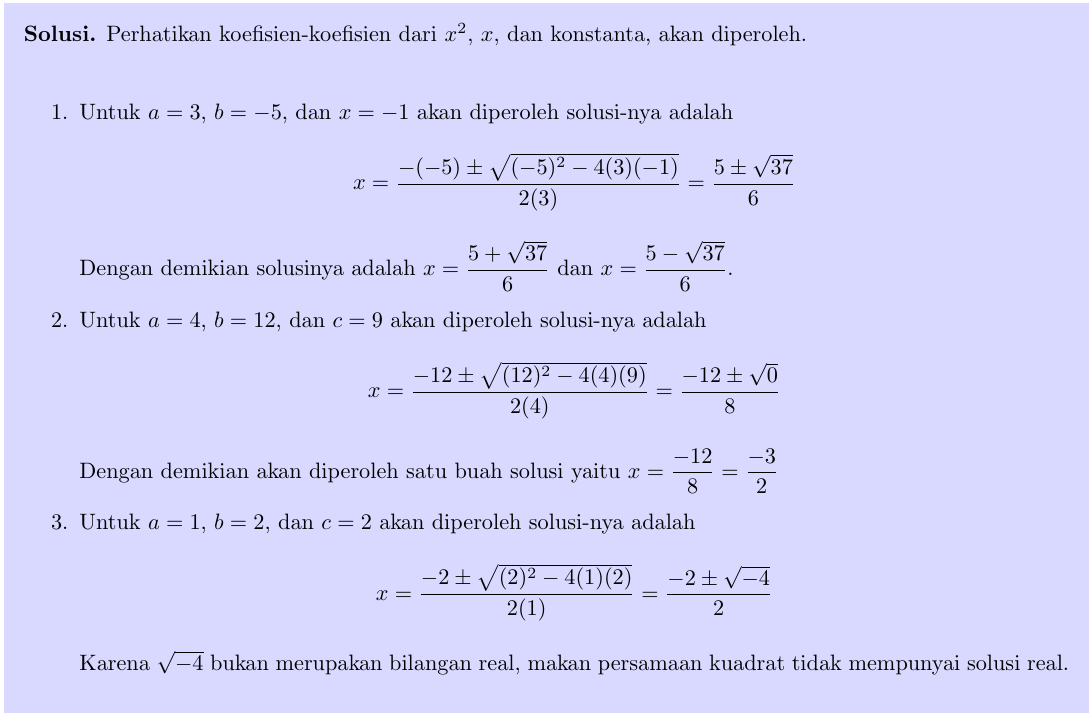
\includegraphics[width=\linewidth]{img/img22}
	\end{center}
\end{frame}

\begin{frame}
	\frametitle{Rumus Persamaan Kuadrat}
	\begin{center}
		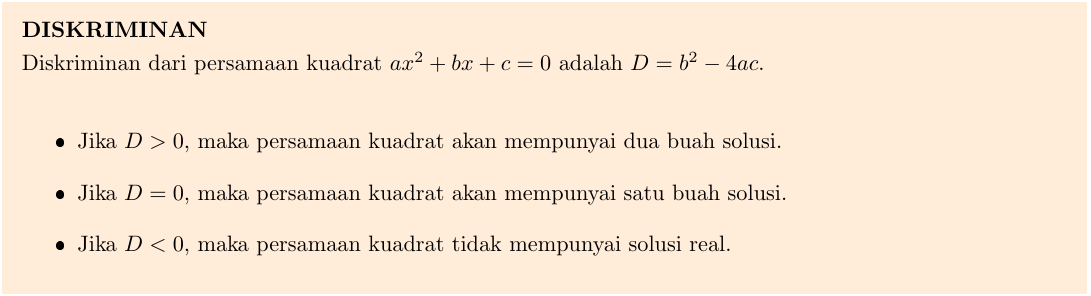
\includegraphics[width=\linewidth]{img/img23}
	\end{center}
\end{frame}

\section{Permodelan Masalah dengan Persamaan}

\begin{frame}
	\frametitle{Permodelan Masalah dengan\\Persamaan}
	\begin{center}
		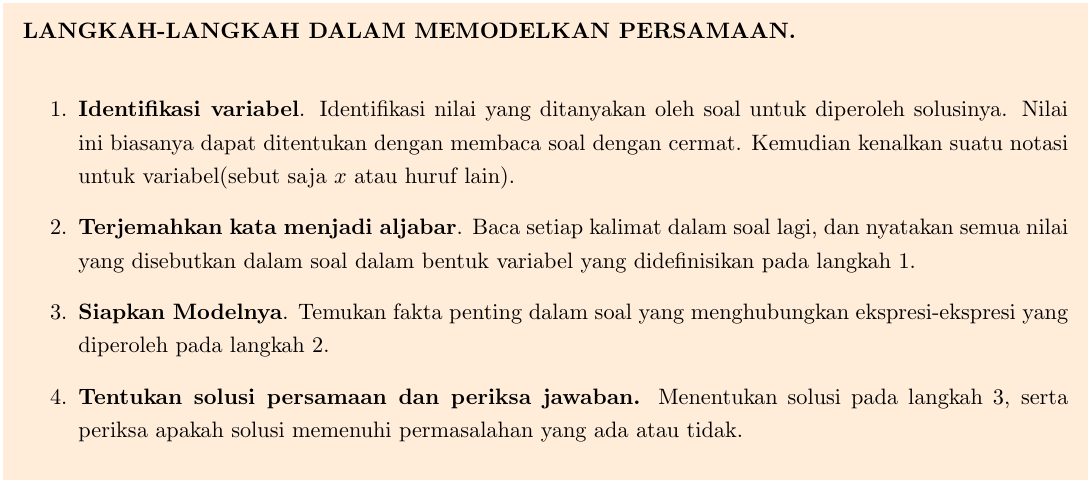
\includegraphics[width=\linewidth]{img/img24}
	\end{center}
\end{frame}

\begin{frame}
	\frametitle{Permodelan Masalah dengan\\Persamaan}
	\begin{center}
		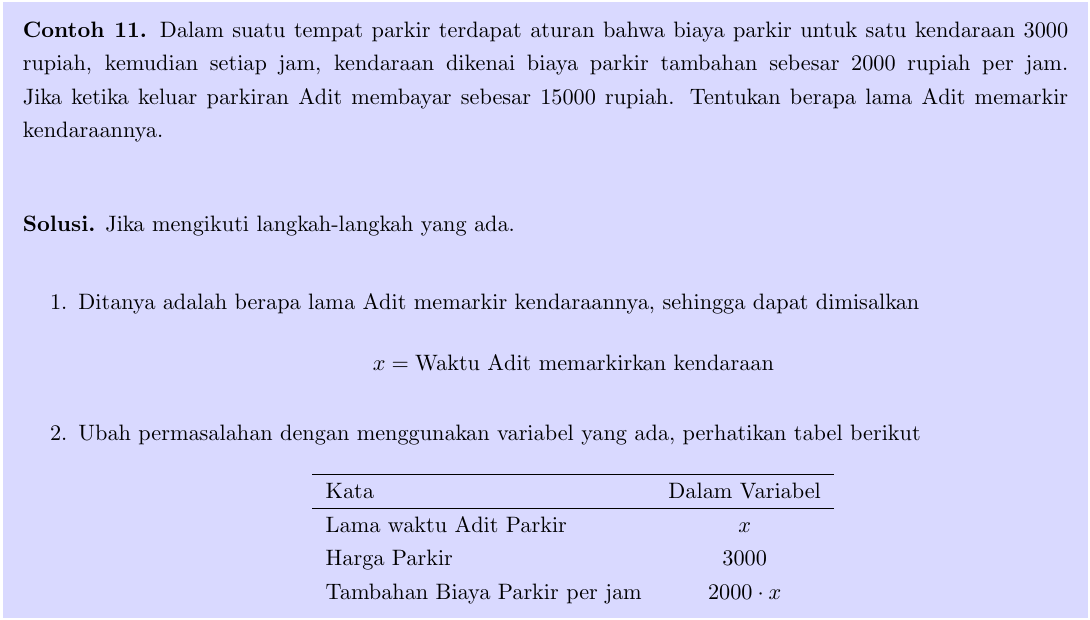
\includegraphics[width=\linewidth]{img/img25}
	\end{center}
\end{frame}

\begin{frame}
	\frametitle{Permodelan Masalah dengan\\Persamaan}
	\begin{center}
		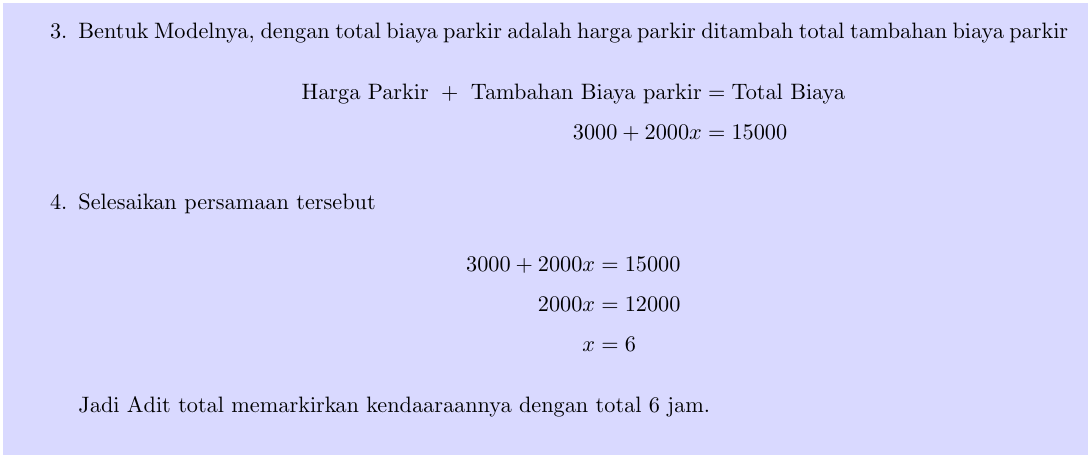
\includegraphics[width=\linewidth]{img/img26}
	\end{center}
\end{frame}

\begin{frame}
	\frametitle{Permodelan Masalah dengan\\Persamaan}
	\begin{center}
		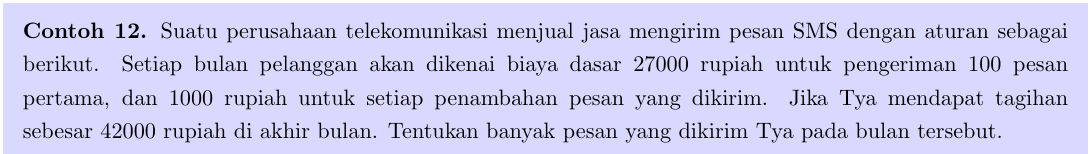
\includegraphics[width=\linewidth]{img/img27}
	\end{center}
\end{frame}

\begin{frame}
	\frametitle{Permodelan Masalah dengan\\Persamaan}
	\begin{center}
		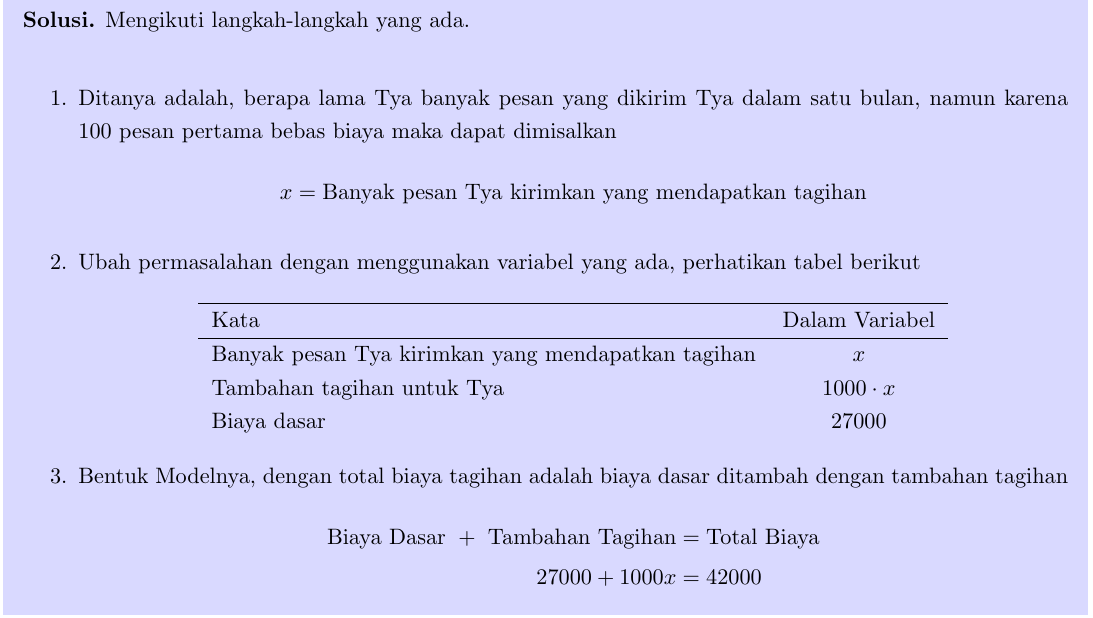
\includegraphics[width=\linewidth]{img/img28}
	\end{center}
\end{frame}

\begin{frame}
	\frametitle{Permodelan Masalah dengan\\Persamaan}
	\begin{center}
		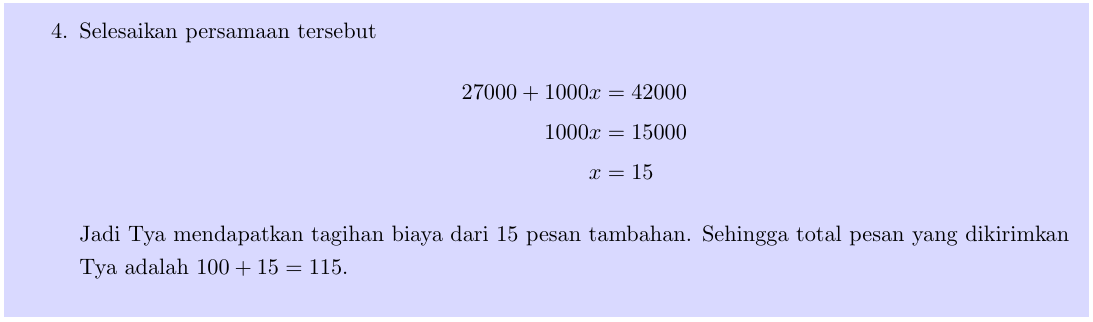
\includegraphics[width=\linewidth]{img/img29}
	\end{center}
\end{frame}

\begin{frame}
	\frametitle{Permodelan Masalah dengan\\Persamaan}
	\begin{center}
		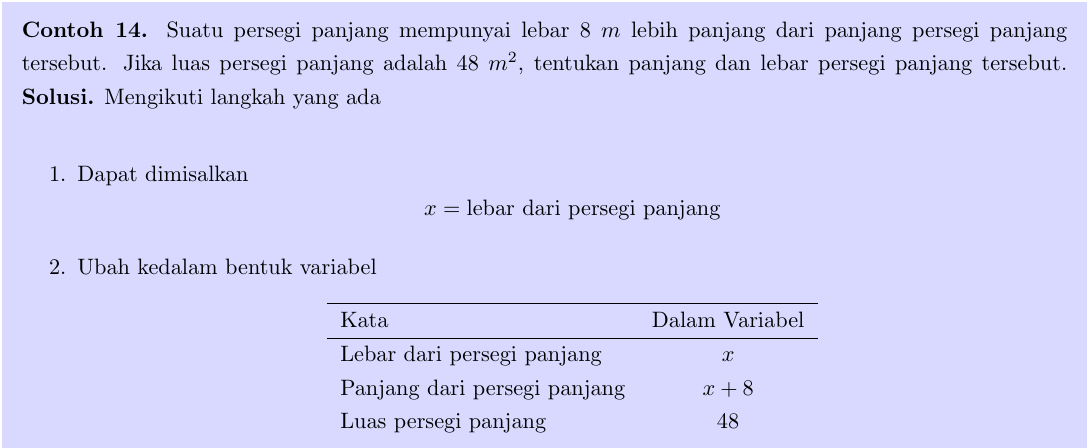
\includegraphics[width=\linewidth]{img/img30}
	\end{center}
\end{frame}

\begin{frame}
	\frametitle{Permodelan Masalah dengan\\Persamaan}
	\begin{center}
		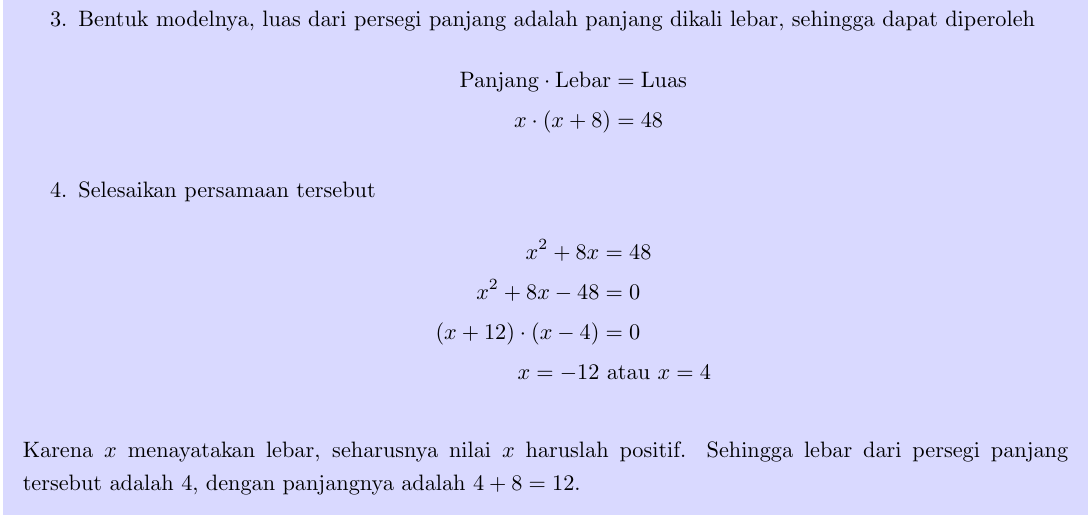
\includegraphics[width=\linewidth]{img/img31}
	\end{center}
\end{frame}

\section{Latihan Soal}

\begin{frame}
	\frametitle{Latihan Soal}
	\begin{center}
		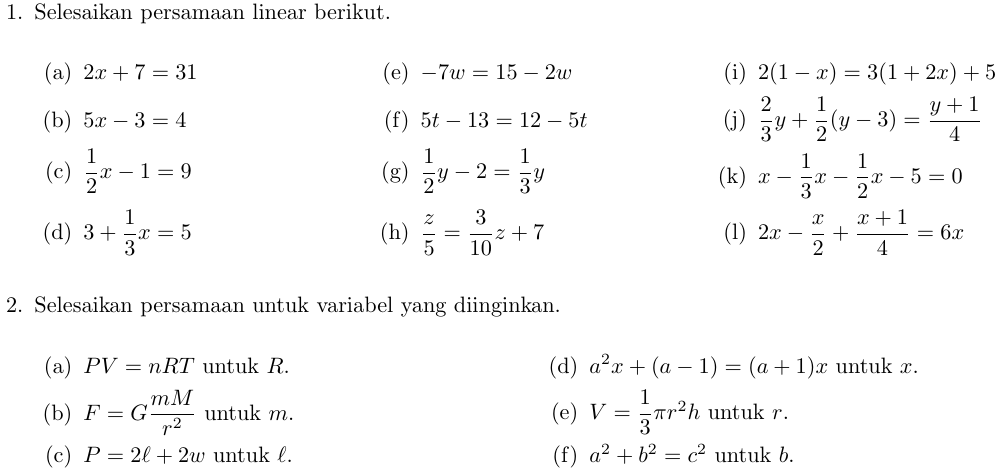
\includegraphics[width=\linewidth]{img/img32}
	\end{center}
\end{frame}

\begin{frame}
	\frametitle{Latihan Soal}
	\begin{center}
		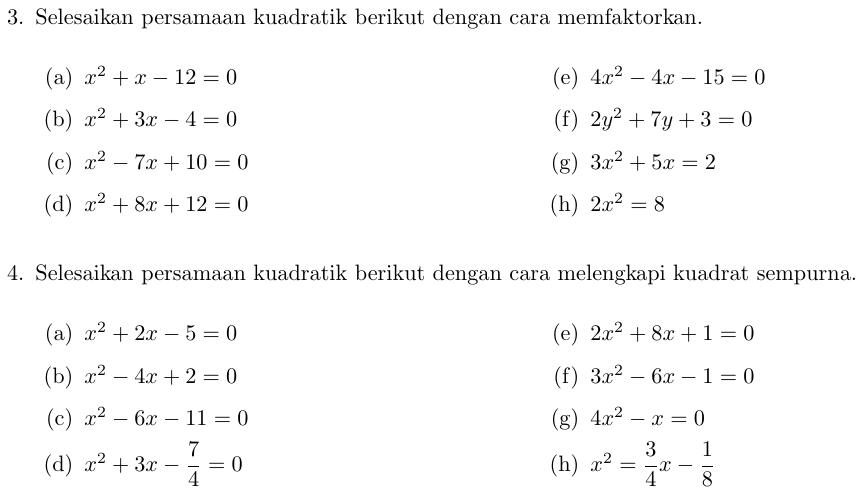
\includegraphics[width=\linewidth]{img/img33}
	\end{center}
\end{frame}

\begin{frame}
	\frametitle{Latihan Soal}
	\begin{center}
		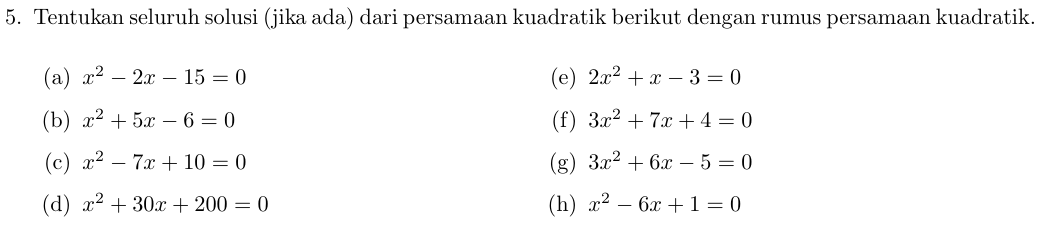
\includegraphics[width=\linewidth]{img/img34}
	\end{center}
\end{frame}

\begin{frame}
	\frametitle{Latihan Soal}
	\begin{center}
		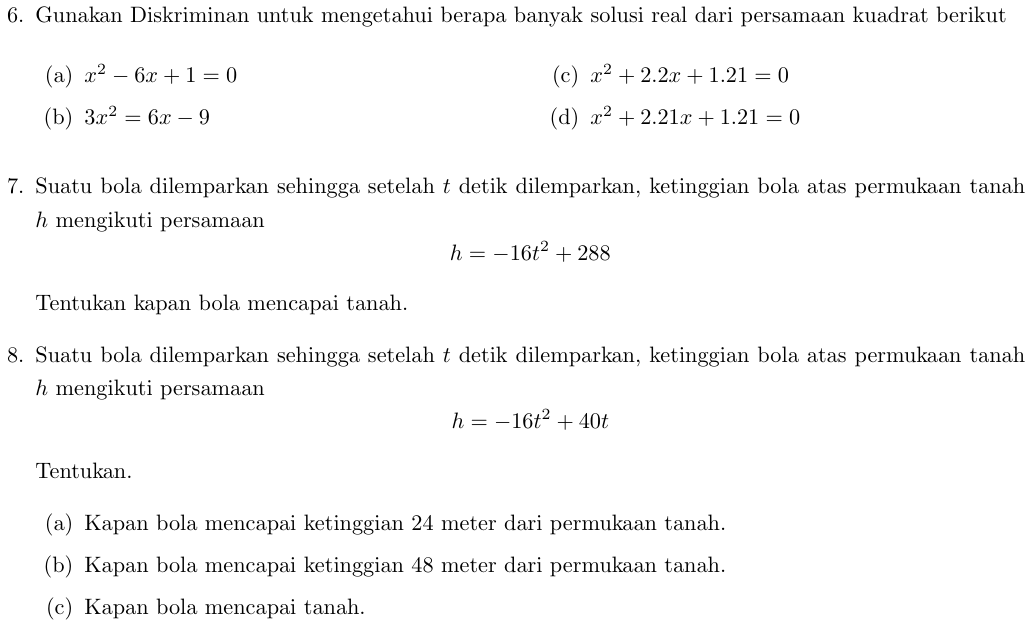
\includegraphics[width=\linewidth]{img/img35}
	\end{center}
\end{frame}

\begin{frame}
	\frametitle{Latihan Soal}
	\begin{center}
		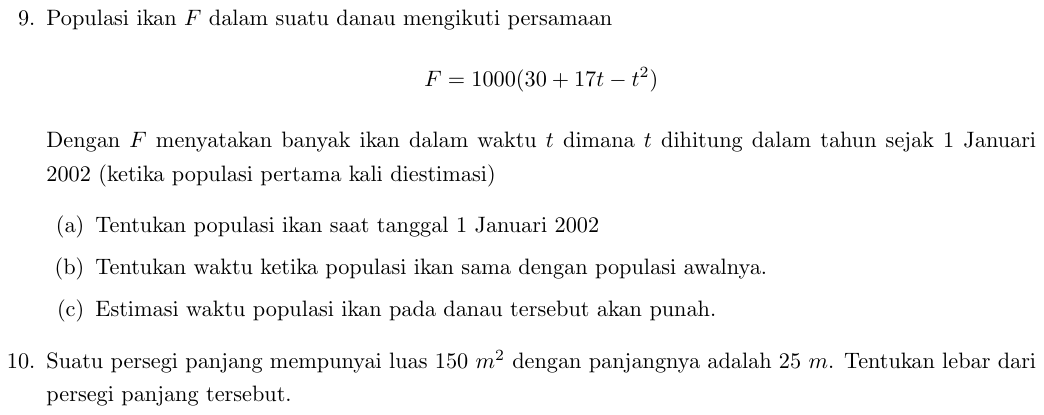
\includegraphics[width=\linewidth]{img/img36}
	\end{center}
\end{frame}

\begin{frame}
	\frametitle{Latihan Soal}
	\begin{center}
		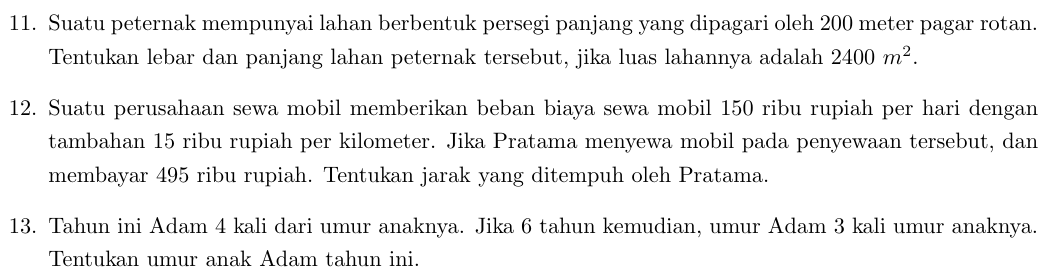
\includegraphics[width=\linewidth]{img/img37}
	\end{center}
\end{frame}

\end{document}
